\section{Preface}

\section{Abstract}

Due to the lack of a net magnetic moment, antiferromagnets possess a unique robustness to external magnetic fields and are thus predicted to play an important role in future magnetic technologies.
However, this robustness also makes them quite difficult to control, and the development of novel methods to manipulate these systems with external stimuli is a fundamental goal of antiferromagnetic spintronics.
In this work, we report evidence for a metastable reorientation of the order parameter in an antiferromagnetic semiconductor triggered by an ultrafast quench of the equilibrium order via photoexcitation above the band gap.
The metastable state forms less than $10$ \si{ps} after the excitation pulse, and persists for longer than $150$ \si{ps} before decaying to the ground state via thermal fluctuations.
Importantly, this transition cannot be induced thermodynamically, and requires the system to be driven out of equilibrium.
Broadly speaking, this phenomenology is ultimately the result of large magnetoelastic coupling in combination with a relatively low symmetry of the magnetic ground state.
Since neither of these properties are particularly uncommon in magnetic materials, the observations presented here imply a generic path toward novel device technology enabled by ultrafast dynamics in antiferromagnets.

\section{Introduction}

When the Hamiltonian of a system contains multiple interaction strengths of comparable magnitude, the corresponding free energy is often host to a diverse collection of metastable states just barely separated in energy from the true ground state.
This phenomenology results in an extreme sensitivity to external stimuli\citep{zhang_dynamics_2014,basov_electrodynamics_2011,dagotto_complexity_2005}, which can be exploited in an ultrafast way using light to drive transitions between these states\citep{basov_towards_2017,kogar_light-induced_2020,mitrano_possible_2016,fausti_light-induced_2011}.

One important application is in magnetic devices, where the electron spins form an ordered state in equilibrium and may thus be used to store information.
\Glspl{afm} have received special attention in this regard, as they possess zero net magnetic moment and are thus robust to stray magnetic fields from adjacent magnetic devices\citep{jungwirth_antiferromagnetic_2016}.
The dominance of exchange rather than anisotropy energies in the dynamics of spins which are antiferromagnetically ordered also leads to order-of-magnitude faster switching timescales compared to their ferromagnetic counterparts\citep{nemec_antiferromagnetic_2018}.

Importantly, the ground state of an \gls{afm} is typically not unique, with the number of degenerate states (corresponding generically to various rotations of the \gls{afm} \gls{op}) being determined by the number of symmetries which are broken at the magnetic ordering temperature.
In the context described above, this degeneracy invites the possibility of an ultrafast antiferromagnetic device which uses light to switch between these different states.
Moreover, if the symmetry of the magnetic phase is sufficiently low (relative to the parent phase), the number of such states can be quite high, and a multi-step magnetic memory might be constructed which operates via ultrafast reorientation transitions of the \gls{afm} \gls{op} between states that are not anti-parallel.

Broadly speaking, one can distinguish two different approaches for achieving such transitions in real materials.
In the first case, one imagines manipulating the \gls{afm} orientation ``coherently'' by, for example, resonantly driving an infrared-active phonon mode to large amplitude, although this usually requires large electric fields (as the relevant light-matter interactions are usually highly nonlinear\citep{afanasiev_ultrafast_2021}) which are difficult to obtain in the frequency range associated with phonons in crystals.
An alternative mechanism -- which has been shown to occur abundantly in \gls{sc}\citep{fausti_light-induced_2011} and \gls{cdw}\citep{kogar_light-induced_2020} systems -- is to \textit{quench} the equilibrium order by exciting carriers above the band gap, and then exploit the subsequent relaxation dynamics which may, in the right system, show a preference for one state over the other\citep{sun_transient_2020}.
In contrast to the case of resonant phonon driving, this mechanism involves primarily electronic excitations and therefore requires relatively little energy if the photon frequency is above the band gap.
However, despite successful demonstrations of this approach in nonmagnetic systems\citep{fausti_light-induced_2011,kogar_light-induced_2020}, evidence for this mechanism occurring in \glspl{afm} does not currently exist, and whether the phenomenology described here actually occurs in real magnetic materials remains a fundamental open question.

In this work, we report a light-induced phase transition between nearly degenerate \gls{afm} states in the antiferromagnetic semiconductor \cmb \citep{gibson_magnetic_2015} triggered by an ultrafast quench of the equilibrium \gls{op} with a femtosecond light pulse.
Using \gls{trshg}, a pump-probe technique with the unique ability to track both the magnitude and direction of the \gls{afm} order parameter as a function of time, we find that above-gap optical excitation indeed causes the system to switch to a new, metastable orientation of the \gls{afm} \gls{op}.
The transition is fast (occurring less than $10$ \si{ps} after photoexcitation), requires low pump fluence (\threshold vs. \previousthreshold\citep{afanasiev_ultrafast_2021}), and cannot be induced thermodynamically.
These findings suggest a new way to manipulate \glspl{afm}, and open the door to novel opto-spintronic device architectures exploiting nonequilibrium phase transitions between different nearly degenerate states. 

\section{Results}

\subsection{Equilibrium}

\begin{figure}
\centering{
\phantomsubfloat{\label{fig0:a}}
\phantomsubfloat{\label{fig0:b}}
\phantomsubfloat{\label{fig0:c}}
\phantomsubfloat{\label{fig0:d}}
}
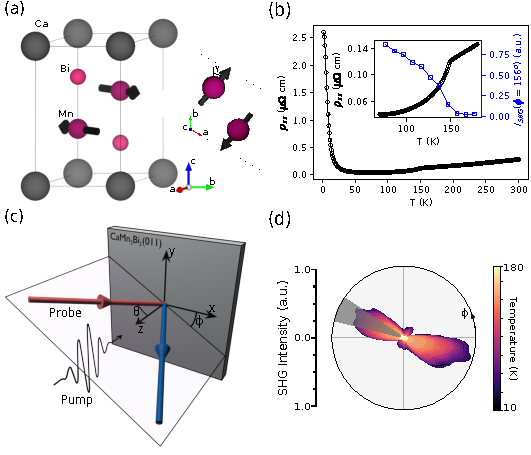
\includegraphics[width=\textwidth]{./gfx/ch6/fig0.pdf}
\captionsetup{singlelinecheck=off}
\caption[]{
\label{fig0}
\begin{enumerate*}[label=\caplabel, ref=\capref]
\item Magnetic unit cell of \cmb.
The angle $\gamma$ is such that the \ce{Mn} spin does not lie precisely along any particular crystallographic axis.
\item Resistivity as a function of temperature for a representative sample.
Inset shows an enlarged view of the resistivity near $T_c$ plotted against the SHG intensity integrated across the region indicated in \ref{fig0:d}.
\item Schematic of the \gls{rashg} setup.
\item Temperature dependence of the \gls{rashg} intensity in the \PP polarization channel from the $(011)$ surface of \cmb.
Other polarization channels are shown in the \sfigonly{\fulltempdep}.
The shaded area indicates the region integrated to produce the inset of \ref{fig0:b}.
\end{enumerate*}
}
\end{figure}

Crystallographically, \cmb consists of a puckered-honeycomb tiling of \ce{Mn} atoms with a high-temperature crystallographic point group of \htpg (see \cref{fig0:a}).
The electronic gap is on the order of $4$ \si{meV} (see \cref{fig0:b}) and is thought to be due to a delicate combination of correlations and hybridization between relatively localized \ce{Mn} $3d$ states and dispersive \ce{Bi} $6p$ / \ce{Mn} $4s$ hybrid bands\citep{gibson_magnetic_2015, piva_putative_2019, lane_competition_2019}.
N\'{e}el-type antiferromagnetic \gls{lro} with spins lying in the $ab$-plane develops in this material at $T_c=\apx150$ \si{K}, accompanied by a kink in the electrical resistivity (\cref{fig0:b}) and the appearance of a new peak in the powder neutron diffraction\citep{gibson_magnetic_2015}.
Importantly, the powder neutron refinement indicates that the ordered moments are slightly misaligned with the $a$- and $b$-axes of the high-symmetry phase (see \cref{fig0:a}), so that the low-temperature magnetic point group is $\bar{1}'$; i.e., the only symmetries that are preserved in the low temperature phase are the identity operator and the product of inversion and time-reversal\citep{gibson_magnetic_2015}.
The remarkably low symmetry of this magnetic ground state is likely due to highly frustrated magnetic interactions, as suggested by to the proximity of isostructural \ce{CaMn2Sb2} to a mean-field magnetic tricritical point\citep{mazin_camn2sb2_2013,mcnally_camn2sb2_2015}.
In contrast, the lattice is thought to remain fully symmetric at all temperatures, so that the symmetry-breaking at $T_c$ is solely due to the \gls{afm} order (this is verified with single-crystal \gls{xrd}, see \supcref{xrd}).

As spin-orbit coupling is expected to be strong in this material, the breaking of inversion symmetry by the magnetic order should result in a strong \gls{shg} signal below $T_c$, despite the fact that the lattice remains centrosymmetric\citep{pan_optical_1989,seyler_spin-orbit-enhanced_2020}.
We probe this \gls{shg} signal using a \gls{rashg} apparatus (\cref{fig0:c}) which measures the reflected second harmonic intensity as the plane of incidence is rotated about the sample normal\citep{fichera_second_2020, harter_high-speed_2015, torchinsky_low_2014}.
\Cref{fig0:b,fig0:d} depict the \gls{shg} signal from the $(011)$ surface of \cmb as a function of temperature across $T_c$, demonstrating that \gls{rashg} is indeed sensitive to the magnetic order in this material.

\begin{figure}
\centering{
\phantomsubfloat{\label{fig1:a}}
\phantomsubfloat{\label{fig1:b}}
\phantomsubfloat{\label{fig1:c}}
\phantomsubfloat{\label{fig1:d}}
\phantomsubfloat{\label{fig1:e}}
\phantomsubfloat{\label{fig1:f}}
\phantomsubfloat{\label{fig1:g}}
}
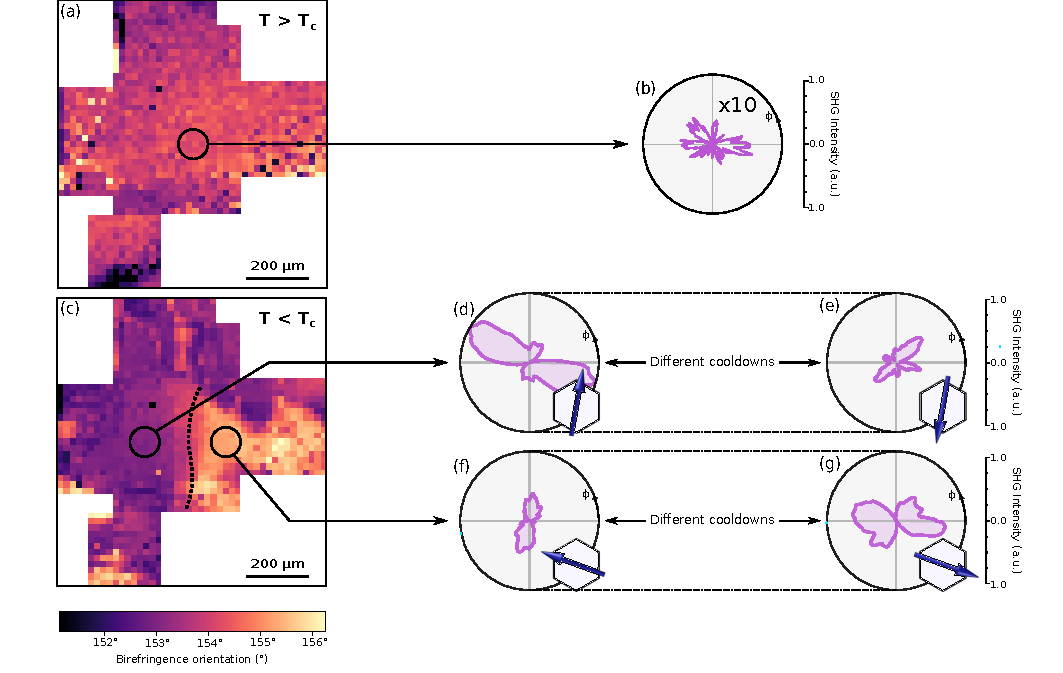
\includegraphics[width=\textwidth]{./gfx/ch6/fig1.pdf}
\captionsetup{singlelinecheck=off}
\caption[]{
\label{fig1}
\begin{enumerate*}[label=\caplabel, ref=\capref]
\item Birefringence orientation map for $T=200~\si{K}>T_c$.
\item \gls{rashg} intensity in the \PP polarization channel for the region indicated in \ref{fig1:a} at $157$ \si{K}.
Other polarization channels are shown in the \supcref{fullequilibrium}.
\item Birefringence orientation map for $T=152.5~\si{K}<T_c$.
\item {} \item \gls{rashg} intensity at $8$ \si{K} in the \PP polarization channel for consecutive cooldowns for the region indicated in \ref{fig1:c}.
The system randomly chooses the \gls{rashg} pattern in \ref{fig1:d} or \ref{fig1:e} on each cooldown.
\insets
Other polarization channels are shown in the \supcref{fullequilibrium}.
\item {} \item \gls{rashg} intensity at $8$ \si{K} in the \PP polarization channel for consecutive cooldowns for the region indicated in \ref{fig1:c}.
The system randomly chooses the \gls{rashg} pattern in \ref{fig1:f} or \ref{fig1:g} on each cooldown.
\insets
Other polarization channels are shown in the \supcref{fullequilibrium}.
The schematic representations beneath the \gls{rashg} plots are for illustration purposes only and the depicted angles are not quantitatively verified.
\end{enumerate*}
}
\end{figure}

Frequently, \gls{afm} materials may host intricate domain configurations, the details of which greatly impact the relevant magnetic functionalities\citep{reimers_defect-driven_2022, weber_magnetostrictive_2003}.
Because the low-temperature magnetic point group of \cmb breaks multiple symmetries of the high-temperature point group, we indeed expect that the low-temperature magnetic ground state should involve some number of energetically degenerate domains.
In \Cref{fig1}, we characterize these domains using a combination of \gls{rashg} and a spatially-resolved optical polarimetry technique known as \gls{ptmb}, which is a sensitive technique for measuring small changes in the anisotropic index of refraction (and consequently, the direction of the \gls{afm} \gls{op})\citep{little_three-state_2020, lee_observation_2022}.

\cref{fig1:a} shows the \gls{ptmb} signal from the $(011)$ surface of \cmb above $T_c$.
No contrast is found within a $\apx500\si{\mu m} \times 500\si{\mu m}$ area on the sample, suggesting that the thermally modulated index of refraction is spatially uniform at high temperature.
As the temperature is lowered below $T_c$ (\cref{fig1:c}), a pronounced contrast appears in the \gls{ptmb} map which indicates the presence of two separate \gls{afm} domains with different \gls{op} directions.

While \gls{ptmb} is nominally sensitive to the direction of the \gls{afm} \gls{op}, it cannot differentiate between $180\degree$ domains as it couples only to the linear index of refraction of the material.
Therefore, it is not clear from \gls{ptmb} alone whether the domains in \cref{fig1:c} are truly homogeneous or may contain a mixture of $180\degree$ domains.
In contrast, nonlinear spectroscopies like \gls{shg} can differentiate $180\degree$ \gls{afm} domains due to an interference between the \gls{shg} sources (e.g. electric dipole, magnetic dipole, and electric quadrupole) which transform differently under time-reversal symmetry\citep{fiebig_second-harmonic_2005, fiebig_second_1994, fiebig_second_2001, fiebig_domain_1995}.
This effect can be especially pronounced in the presence of magnetostriction\citep{fiebig_second_2001}.
We thus proceed to investigate the presence of $180\degree$ domains in this material using \gls{rashg}.

\crefrange{fig1:d}{fig1:g} depict the \gls{rashg} results at $8$ \si{K} in the two regions identified in \cref{fig1:c}.
The same crystal piece was used for both measurements.
As with \gls{ptmb}, we do find that the \gls{shg} domains are large and apparently homogenous (on a scale of hundreds of \si{\mu m}).
Surprisingly, however, in different cooldowns we observe that the \gls{rashg} pattern in the leftmost region of \cref{fig1:c} randomly takes the form of either \cref{fig1:d} or \cref{fig1:e}, and in the rightmost region, it takes the form of either \cref{fig1:f} or \cref{fig1:g}.
In contrast, the \gls{ptmb} does not change upon thermal cycling.
Anticipating again that \gls{rashg} should be sensitive to the phase of the \gls{afm} \gls{op} as well as its direction, we interpret \cref{fig1} as follows: \cref{fig1:d} and \cref{fig1:e} correspond to opposite $180\degree$ \gls{afm} domains, as do \cref{fig1:f} and \cref{fig1:g}; in addition, there is a relative angle between \crefrange{fig1:d}{fig1:e} and \crefrange{fig1:f}{fig1:g}, as indicated by the \gls{ptmb}.
This interpretation is depicted schematically in the insets to \crefrange{fig1:d}{fig1:g}, where the \gls{afm} \gls{op} (defined as the difference in the magnetic moment on the two \ce{Mn} sublattices, see \cref{fig0:a}) is represented by a blue arrow.
Importantly, within a single location, the two opposite orientations are accessible via thermal cycling; hence they are energetically degenerate.
We have verified that the identification described here is consistent with the \gls{shg} susceptibility tensors\citep{boyd} extracted by fitting the data in \cref{fig1} (see \supcref{sec:fitting}).
In addition, the data presented in \cref{fig1} is not consistent with an alternative interpretation involving the interference of two independent order parameters (see \supcref{sec:alternativeinterpretation}).

\subsection{nonequilibrium}
\begin{figure}
\centering{
\phantomsubfloat{\label{fig2:a}}
\phantomsubfloat{\label{fig2:b}}
\phantomsubfloat{\label{fig2:c}}
\phantomsubfloat{\label{fig2:d}}
}
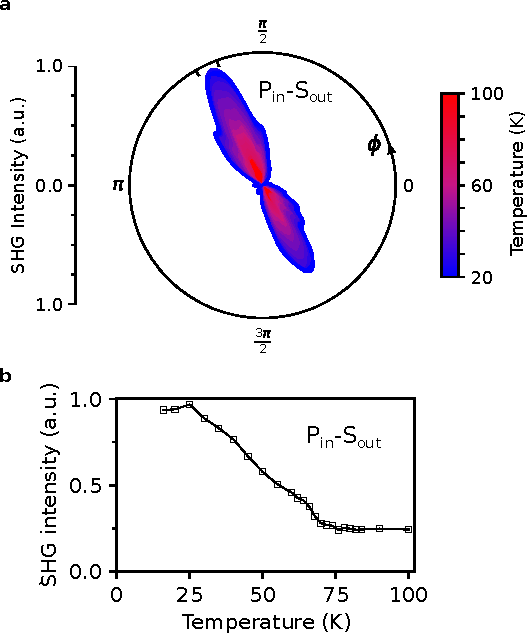
\includegraphics[width=\textwidth]{./gfx/ch6/fig2.pdf}
\captionsetup{singlelinecheck=off}
\caption[]{
\label{fig2}
\begin{enumerate*}[label=\caplabel, ref=\capref]
\item[] \gls{rashg} intensity at $8$ \si{K} in the \PP polarization channel as a function of time for the \gls{afm} \gls{op} identified in \item \cref{fig1:d}, \item \cref{fig1:e}, \item \cref{fig1:f}, and \item \cref{fig1:g}.
The pump fluence is set to $\apx 600$ \si{\mu J \cdot cm^{-2}}.
\insets
Other polarization channels are shown in the \supcref{fullnonequilibrium}.
The schematic representations beneath the \gls{rashg} plots are for illustration purposes only and the depicted angles are not quantitatively verified.
\end{enumerate*}
}
\end{figure}

Having demonstrated that \cmb hosts an elaborate free energy surface with multiple degenerate or nearly degenerate ground states, we now turn to the question of whether light can be used to manipulate or possibly switch between these states. 
To answer this question, we pump each of the \gls{op} directions identified in \cref{fig1} at $8$ \si{K} with a $\apx 100$ \si{fs} normally incident near-infrared light pulse ($\hbar \omega \approx 1$ \si{eV}) and probe the \gls{afm} \gls{op} with \gls{rashg} using a subsequent probe pulse.
By varying the delay $\Delta t$ between the two pulses, we create a series of snapshots of the \gls{afm} \gls{op} at different times following excitation.
The results are shown in \cref{fig2}, where the four rows correspond to the four \gls{op} directions identified in \cref{fig1}, and the horizontal axis is the time delay between the pump and probe pulses.
The first two rows (\crefrange{fig2:a}{fig2:b}) correspond to the leftmost domain in \cref{fig1:c}, for which it is found that, after pumping, the strength of the \gls{rashg} signal is quickly extinguished.
After a delay of around $\apx 8-10$ \si{ps}, the \gls{afm} order recovers so that the shape of the \gls{rashg} pattern is similar to before zero delay up to small changes in the relative peak heights.
The \gls{op} magnitude and direction inferred by this data is depicted schematically in the insets to \crefrange{fig2:a}{fig2:b}.

The striking observation is in the latter two rows (\crefrange{fig2:c}{fig2:d}), which depict the time-resolved \gls{rashg} results in the rightmost domain of \cref{fig1:c}.
In this domain, the \gls{rashg} signal again quickly decreases, and the shape does not initially change.
However, roughly $\apx 6-8$ \si{ps} after excitation, the \gls{rashg} pattern abruptly changes shape, so that the pattern after $\apx 10$ \si{ps} is equivalent to \cref{fig2:a}.
Together with the findings of \cref{fig1}, these results suggest that the final state in \crefrange{fig2:c}{fig2:d} is one in which the \gls{afm} \gls{op} direction has indeed been reoriented relative to equilibrium.
Remarkably, one must use light to reach this metastable state as it is not present in thermal equilibrium at this spot.

\begin{figure}
\centering{
\phantomsubfloat{\label{fluencedep:a}}
\phantomsubfloat{\label{fluencedep:b}}
}
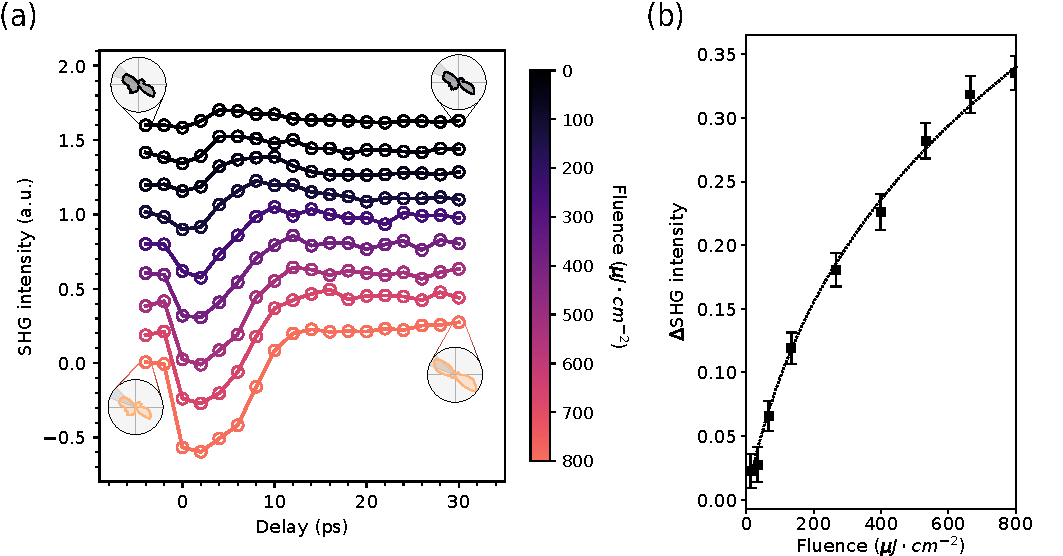
\includegraphics[width=\textwidth]{./gfx/ch6/fluencedep.pdf}
\captionsetup{singlelinecheck=off}
\caption[]{
\label{fluencedep}
\begin{enumerate*}[label=\caplabel, ref=\capref]
\item Integrated SHG intensity for a representative \gls{afm} domain as a function of delay and pump fluence.
Insets show the initial (left) and final (right) states at high (bottom) and low (top) pump fluences, as well as the integration region (indicated by the shaded area).
\item Difference between the intensity of the integration region specified in \ref{fluencedep:a} at long times (averaged from $\Delta t=40$ to $\Delta t=50$ \si{ps}) and the intensity before zero delay (averaged from $\Delta t=-4$ to $\Delta t=-2$ \si{ps}).
Dashed line is a guide to the eye.
\end{enumerate*}
}
\end{figure}

We performed the above measurements out to $\Delta t \gtrsim 150$ \si{ps} (see \supcref{CtoBlong}) and found that the reoriented state persists at least this long before relaxing back to equilibrium in time for the next pair of pulses to arrive (roughly $200$ \si{\mu s} later).
As the pump fluence is decreased (see \supcref{fluencedep}), the effect of the excitation is diminished until, at low fluences ($\apx 100$ \si{\mu J \cdot cm^{-2}}), the final state is equivalent to the initial state, and only small changes to the \gls{shg} (associated with dynamics that do not launch the system into the metastable state) are visible near zero delay.
Interestingly, which of the two opposite directions (\cref{fig1:d} or \cref{fig1:e}) the magnetic order favors after excitation is consistent from pulse to pulse, but not from one sample to another (see \supcref{CtoBshort,CtoBlong}), suggesting that, below the magnetic ordering temperature, interactions between neighboring domains break the degeneracy between these states.
Finally, we note that no aspect of these observations changes with the polarization of the pump pulse (see \supcref{polarization}).

\section{Discussion}

Taken together, these considerations indeed point to a \textit{bona fide} ultrafast phase transition in \cmb induced by a femtosecond light pulse.
We now seek to understand, at least qualitatively, the microscopic nature of this transition.
Before discussing the time-resolved data of \cref{fig2}, we must first understand the equilibrium phenomenology implied by \cref{fig1}.
Group theory (see \supcref{sec:nonequilibriumtheory}) suggests that there should be twelve energetically degenerate \gls{op} directions, independent of location on the sample.
However, only two directions are observed per measurement location in our experiment.
This observation is explained by recognizing that local strain fields in the material are expected to pole the \gls{lro} (see \supcref{sec:equilibriumtheory}), so that certain \gls{op} directions are energetically favored relative to others at a given spot\citep{higo_perpendicular_2022,ni_imaging_2021}.
Since these strain fields may vary from one location to another (the details of which depend subtly on the local growth conditions), different locations on the sample would then show different sets of \gls{rashg} patterns, in agreement with the findings of \cref{fig1}.
This picture also explains the observation that opposite \gls{afm} configurations are energetically degenerate, as strain itself is inherently symmetric under $180^\circ$ rotations.

\begin{figure}
\centering{
\phantomsubfloat{\label{fig3:a}}
\phantomsubfloat{\label{fig3:b}}
\phantomsubfloat{\label{fig3:c}}
\phantomsubfloat{\label{fig3:d}}
\phantomsubfloat{\label{fig3:e}}
}
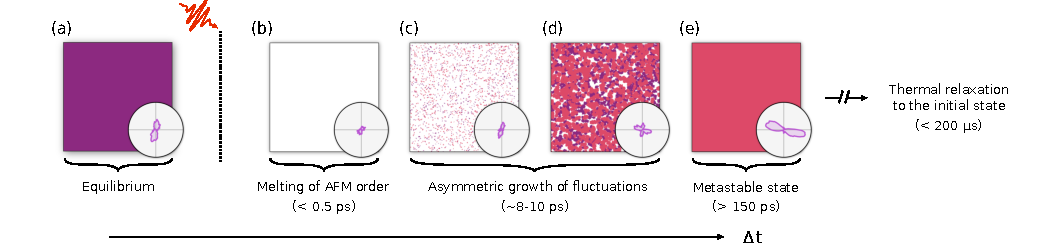
\includegraphics[width=\textwidth]{./gfx/ch6/fig3.pdf}
\captionsetup{singlelinecheck=off}
\caption[]{
\label{fig3}
\begin{enumerate*}[label=\caplabel, ref=\capref]
\item[] Illustration of the dynamics following laser excitation as described in the text.
Ultrafast melting of the \gls{afm} order (\ref{fig3:a}-\ref{fig3:b}) is followed by the rapid growth of fluctuations (\ref{fig3:c}-\ref{fig3:d}), with the final state (\ref{fig3:e}) determined by the relative growth rate of different orders.
The fluctuation growth step (\ref{fig3:c}-\ref{fig3:d}) may occur with or without a background of coherent oscillations (see \supcref{sec:fluctuations,sec:nonequilibriumtheory}).
\end{enumerate*}
}
\end{figure}

Turning now to the nonequilibrium phenomenology (\cref{fig2,fig3}), we begin by noting that the sudden suppression of the \gls{shg} intensity at early times indicates that the primary effect of the pump pulse is simply to quench the \gls{afm} \gls{op} (\cref{fig3:a,fig3:b}).
According to recent theoretical work \citep{sun_transient_2020, dolgirev_self-similar_2020}, the dynamics following such a quench are governed not by the global minimum of the free energy, but rather by the exponential amplification of spatial \gls{op} fluctuations (\cref{fig3:c,fig3:d}), which may occur differently for different orders (\supcref{sec:fluctuations}).
The final state of the transition (\cref{fig3:e}) is then determined by which state supports the fastest-growing fluctuations.
In the context of light-induced \gls{sc}\citep{fausti_light-induced_2011,cremin_photoenhanced_2019}, for example, the dominant order in equilibrium is a \gls{cdw}, whose fluctuations naturally involve motion of the massive nuclei and are thus much slower than fluctuations of the \gls{sc} \gls{op}\citep{smallwood_tracking_2012,sun_transient_2020}.
Note that, in the general case, the final state is determined not just by the relaxation rates, but also by their start times; that is, if one order is \textit{quenched} faster than another, fluctuations of that order are afforded a longer period to grow and may thus dominate at long times.

In our system, the relatively slow ($\apx 8-10$ \si{ps}, see \cref{fig2}) recovery timescale indicates that the dynamics of the \gls{afm} \gls{op}, like the \gls{cdw} order of \citet{fausti_light-induced_2011}, also likely involve motion of the atomic nuclei (i.e. magnetoelastic coupling).
However, in contrast to the \gls{cdw}-\gls{sc} competition referred to above, the dominant and subdominant orders in our system correspond not to completely different orders, but rather to different orientations of the same order.
One would thus naively expect the corresponding fluctuations to exhibit more or less the same dynamics.
However, as described above, this naive symmetry of the material is in fact broken at all temperatures by the internal strain; thus, it is appropriate to think of the two non-parallel \gls{afm} orientations as truly distinct orders.
Importantly, it is noted in \citet{sun_transient_2020} that small variations in the density of different fluctuations are exponentially amplified as the system relaxes, so that only a modest difference in the relevant dynamics is sufficient to favor the metastable state as the system recovers.
Such asymmetric amplification of non-parallel \gls{afm} orientations thus likely forms the basis for the reorientation transition in \cmb.

\begin{figure}
\centering
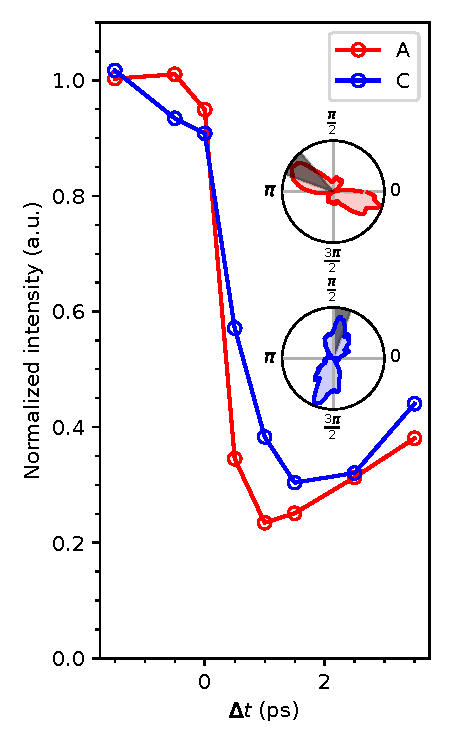
\includegraphics[width=\textwidth]{./gfx/ch6/quenchtimes.pdf}
\captionsetup{singlelinecheck=off}
\caption[]{
\label{quenchtimes}
Integrated \gls{shg} intensity as a function of time corresponding to \cref{fig3:a} (A, red) and \cref{fig3:c} (C, blue).
Insets show the equilibrium \gls{shg} patterns in the \PP polarization combination for the two domains, with the integration region indicated in gray.
The $y$-axis normalization for either domain is defined such that the average signal before zero delay equal to $1.0$.
}
\end{figure}

Evidence supporting this picture may be found by examining the time dependence of the \gls{shg} signal at short times (\supcref{quenchtimes}), before the \gls{op} switches to the metastable state.
In particular, on examining the initial decay rates it can be seen that the \gls{shg} signal corresponding to \cref{fig2:a} reaches $30\%$ of its original value just $0.5$ \si{ps} after zero delay; the equivalent drop in \gls{shg} intensity for \cref{fig2:c} takes $> 0.5$ \si{ps} longer.
That is, the quench dynamics associated with the metastable state are roughly twice as fast as those associated with the equilibrium state.
As a result, long-wavelength fluctuations of the subdominant, metastable order experience a longer period of exponential amplification compared to the equilibrium order, which may explain the dominance of the metastable state at long times.
The metastability of the final state is provided by the fact that the long-term relaxation dynamics are presumably dependent on the thermal nucleation and subsequent motion of \gls{afm} domain walls, which can be quite slow\citep{parkin_memory_2015,kim_real-space_2022}.
Finally, we remark that while the quench dynamics described here can explain all features of our data, they also likely occur alongside a background of coherent excitations (e.g. coherent phonons, which are observable in time-resolved reflectivity, see \supcref{pp}) which can couple to the order parameter via the lattice strain (see \supcref{sec:nonequilibriumtheory}).
While no evidence of these excitations is apparent in our \gls{shg} data, further studies will be needed to determine the extent to which they might still be important.

\section{Conclusion}

To summarize, we have presented evidence of a magnetic reorientation transition in the antiferromagnetic semiconductor \cmb induced by above-gap optical excitation.
Looking forward, we note two ingredients that seem to be most important for the transition demonstrated in this work: low symmetry, so that there are multiple energetic minima in the magnetic phase, and, presumably, some degree of magnetoelastic coupling, so that the different minima are not precisely degenerate in thermal equilibrium.
Neither of these properties are unique to \cmb, and analogous materials may exist with similar light-induced phenomenology. 
The apparently pronounced coupling between light and magnetic order in this material also invites the fascinating possibility that the magnetic order could be manipulated via additional tuning parameters like strain or current.
This is a key prediction of so-called \pt-symmetric systems, in which inversion and time-reversal symmetries are independently broken but the product of the two is preserved\citep{watanabe_group-theoretical_2018, watanabe_nonlinear_2020, watanabe_symmetry_2018}.
Further investigation of these and related compounds could have far-reaching impacts for future opto-spintronic technology.

\section{Methods}

\subsection{Material growth}

Single crystals of \cmb were grown by a \ce{Bi} flux method following \citet{gibson_magnetic_2015}.
The starting materials were \ce{Ca} ingot, \ce{Mn} powder, and \ce{Bi} powder.
They were loaded into an alumina crucible in the molar ratio of $\ce{Ca}:\ce{Mn}:\ce{Bi} = 1:2:10$, which was sealed in an evacuated quartz tube.
The ampoule was heated to $1000^\circ$\si{C} and kept at this temperature for $11$ hours before being slowly cooled to $400^\circ$\si{C} in $10$ days.
The excess flux was removed by a centrifuge at this temperature.
The single phase nature of the crystals was checked by powder \gls{xrd} and the orientation was checked by a single-crystal x-ray diffractometer.

\subsection{\gls{trshg} measurements}

The \gls{trshg} measurements were performed using a fast-rotating optical grating method which has been described previously\citep{fichera_second_2020, harter_high-speed_2015, torchinsky_low_2014}.
Ultrashort ($\apx 100$ \si{fs}) probe pulses were sourced from a regeneratively amplified \ce{Ti}:Sapphire laser operating at a repetition rate of $5$ \si{kHz}.
A portion of the \ce{Ti}:Sapphire output was directed to an optical parametric amplifier, producing $\apx 1$ \si{eV} pump pulses which were delayed relative to the probe pulses with an optical delay line.
The incident probe fluence was $\apx 250$ \si{\mu J \cdot cm^{-2}}, with the probe spot diameter being $\apx 100$ \si{\mu m} at the sample surface, and the pump pulses (with varying fluence) were focused to a spot roughly $\apx 400$ \si{\mu m} in diameter.
The pump was normally incident to the sample surface, but the probe was incident with an angle of $\apx 10^\circ$.
The reflected \gls{shg} signal was collected with a photomultiplier tube, filtered with a lock-in amplifier operating at the repetition rate of the regenerative amplifier, and correlated with the rotation angle of the grating with an optical rotary encoder and homebuilt oscilloscope.
To eliminate potential artifacts due to low-frequency fluctuations in the laser intensity, multiple random sweeps of the delay stage were averaged together for each dataset, and the polarizers were controlled automatically at each delay using custom polarization rotators described in \citet{morey_in_prep}.

\subsection{\gls{ptmb} measurements}

The polarization-dependent optical birefringence (linear dichroism) measurements were conducted using the experimental setup detailed in \citet{little_three-state_2020}.
A $633$ \si{nm} probe laser beam was focused onto a $5$ \si{\mu m} spot at surface of the sample, while a $780$ \si{nm} pump/heating beam was similarly focused onto the same location.
To improve the signal-to-noise ratio and eliminate polarization artifacts originating from the experimental setup, the sample temperature was modulated at $2$ \si{kHz} by passing the pump beam through an optical chopper.
The linear dichroism signal was subsequently measured using a standard balanced photodetection scheme and a lock-in amplifier.
Position-dependent measurements of optical birefringence were obtained by scanning the sample position with a piezoelectric scanner.
The dependence of the polarization rotation on the probe polarization angle was fit to a sinusoidal function at each spot, and the phase shift parameter extracted from each fit was plotted in \cref{fig1:a,fig1:c}.
Note that the birefringence signal involves contributions from both the lattice and the magnetism, so that the angle extracted from this fit should not be identified with the angle of the \gls{afm} \gls{op}.

\subsection{\gls{xrd} measurements}

\Gls{xrd} data (\supcref{xrd}) were collected at $100$ \si{K} and $180$ \si{K} on a Bruker-AXS X8 Kappa Duo diffractometer with I\textmu S micro-sources, coupled to a Photon 3 CPAD detector using \si{Mo} K\textalpha~radiation ($\lambda = 0.71073$ \si{\angstrom}), performing $\phi$-and $\omega$-scans. 
Reconstructed precession images of the $(0kl)$, $(h0l)$ and $(hk0)$ planes were calculated directly from the diffraction images using algorithms included in the APEX3\citep{apex} software.  

\subsection{Data availability}

Data supporting the figures within this paper and other findings of this study are available from the corresponding author upon request.

\section{Acknowledgments}

The authors thank Clifford Allington, Martin Eckstein, Shiang Fang, Feng Hao, David Hsieh, Honglie Ning, Jia Xu, and Guangua Zhang for several helpful discussions.
The authors also acknowledge the MIT SuperCloud and Lincoln Laboratory Supercomputing Center for providing HPC resources that have contributed to the research results reported within this paper.
B.F., B.L., K.M., Z.S., B.I., T.L., and N.G. acknowledge support from the US Department of Energy, BES DMSE (data taking and analysis), and Gordon and Betty Moore Foundation’s EPiQS Initiative grant GBMF9459 (instrumentation).
C.L., E.D., A.L.-P., and J.O. acknowledge support from the Quantum Materials program under the Director, Office of Science, Office of Basic Energy Sciences, Materials Sciences and Engineering Division, of the US Department of Energy, Contract No. DE-AC02-05CH11231.
G.A.F. gratefully acknowledges support from the NSF through the Center for Dynamics and Control of Materials: an NSF MRSEC under DMR-1720595, NSF DMR2114825, and the Alexander von Humboldt Foundation.
R.H.A.d.T., M.A.,A.L., and A.A. acknowledge support from the Spanish Ministry of Science and Innovation through grants PID2019-105488GB-I00, TED2021-132074B-C32 and PID2022-PID2022-139230NB-I00, the European Commission from the MIRACLE (ID 964450), and the Basque Government through Project No. IT-1569-22.

\section{Supplementary Material}

\subsection{Supporting theoretical discussion}

\subsubsection{Equilibrium strain-spin coupling}\label{sec:equilibriumtheory}

To study the coupling between intrinsic strain and magnetic order in \cmb, theoretical calculations were performed using the \gls{paw} implemented in the \gls{vasp}\citep{kresse_efficient_1996, kresse_from_1999}.
For the exchange and correlation potential, we use the Perdew-Burke-Ernzerhof form of the \gls{gga}, which is further corrected with the Couloumb U parameter following the \gls{gga}+U formulation of Dudarev\citep{dudarev_electron-energy-loss_1998}.
We perform a test calculation of the \gls{pdos} using the HSE06 hybrid functional.
Comparing this with the \gls{gga} and \gls{gga}+U calculations, we determine that for an improved system description, it is necessary to include the terms $U(\ce{Mn})=4$ \si{eV} and $U(\ce{Bi})=3$ \si{eV}.
All calculations were performed with a well-converged plane-wave cutoff energy of $700$ \si{eV}, a gamma-centered $15\times15\times8$ Monkhorst-Pack $k$-point mesh, and a Fermi smearing of $20$ \si{meV}.
Atomic coordinates were relaxed until forces in all directions were smaller than $0.5$ \si{meV/\r{A}}.
An energy convergence criterion of $10^{-7}$ \si{eV} is used.
The atomic valence configuration for Ca, Mn and Bi are 3$s^2$3$p^6$4$s^2$4$p^{0.01}$, 4$s^2$3$d^5$ and 6$s^2$6$p^3$, respectively.
The ground state in the trigonal unit cell shows \gls{afm} order between the Mn atoms with an energy difference of about $200$ \si{meV}.

\begin{figure}
\centering
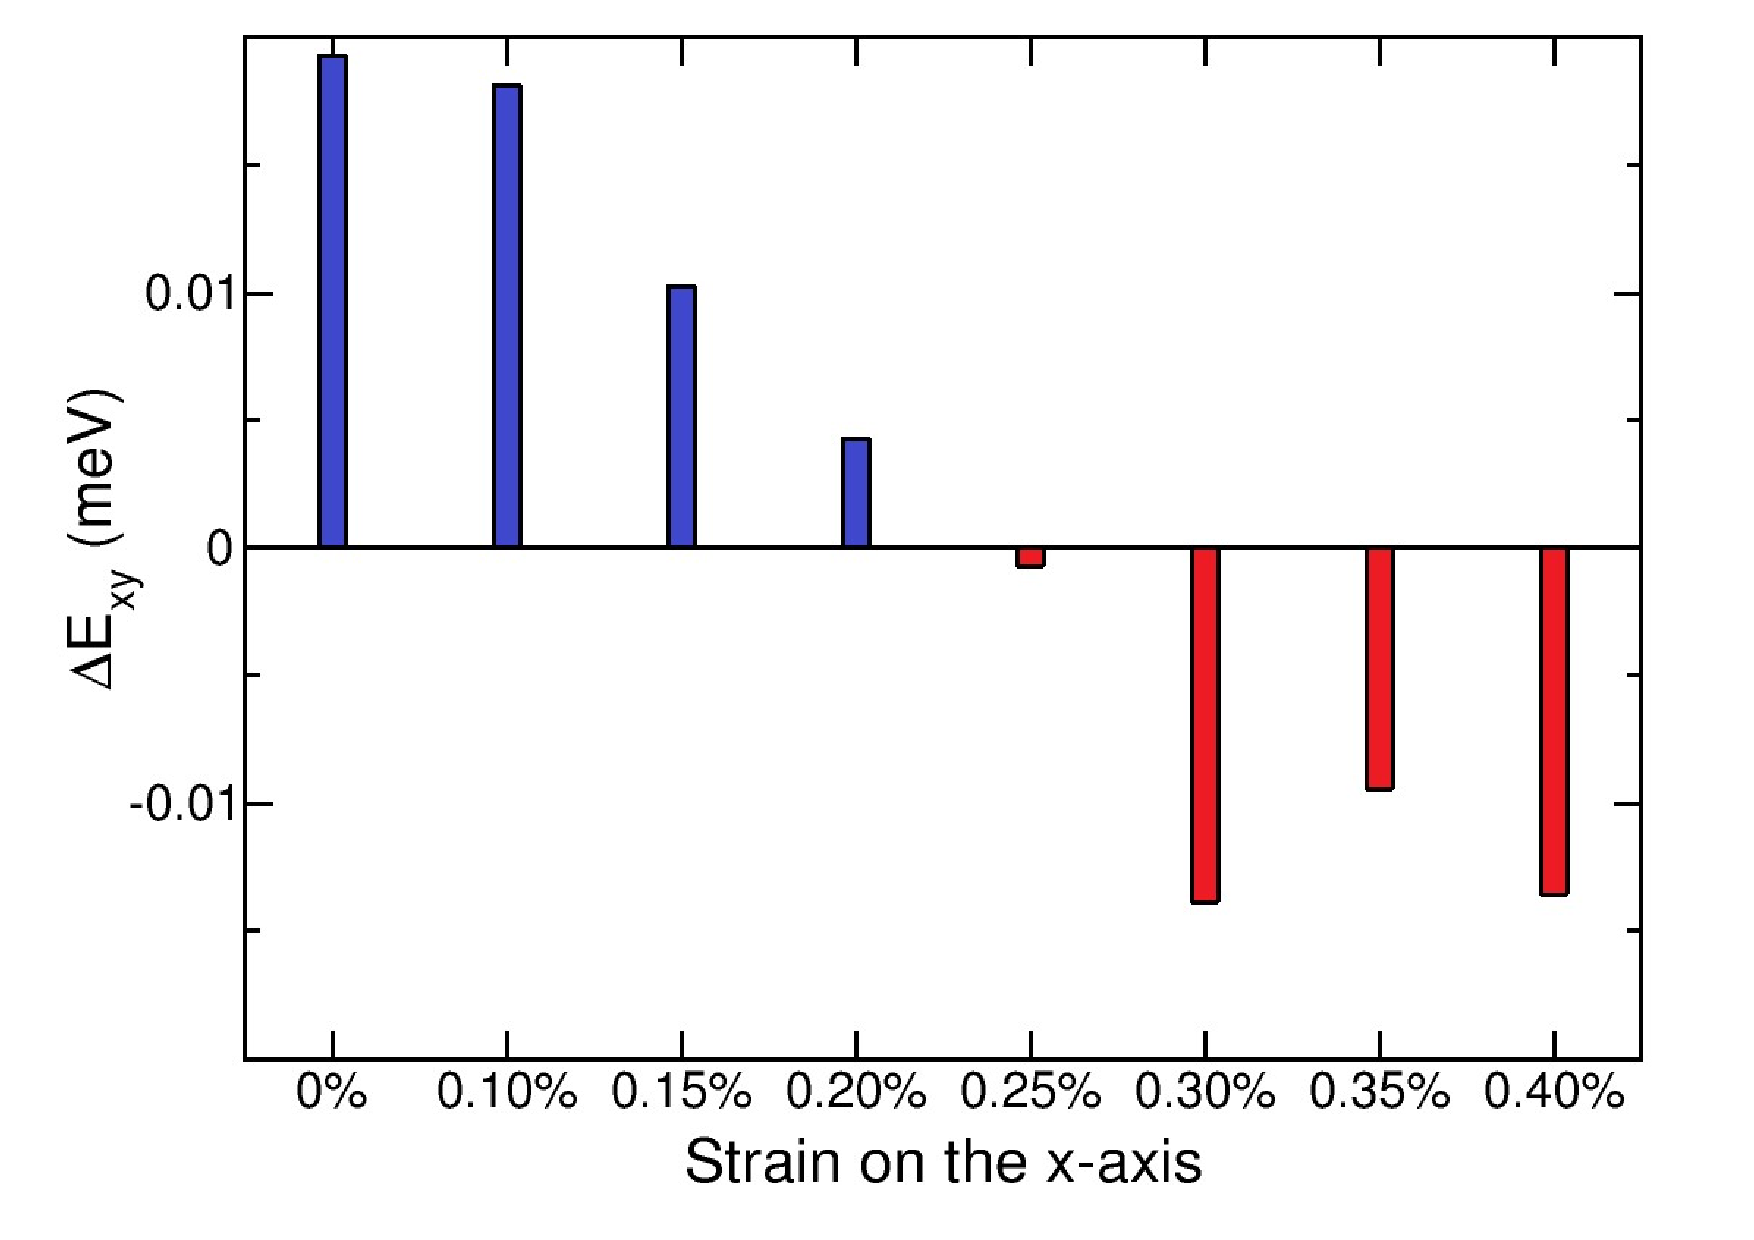
\includegraphics[width=\textwidth]{./gfx/ch6/equilibriumtheory.pdf}
\caption{
\label{fig:equilibriumtheory}
Energy difference between $x$ and $y$-directions with respect to the easy axis.
Blue bars indicate the $x$-direction for the \gls{afm} \gls{op} is preferred, and red bars indicate the $y$-direction for the \gls{afm} \gls{op} is preferred.
Note that for strains in experiments, the difference value goes to zero, indicating a change in the in-plane magnetic moment direction.
}
\end{figure}

By including the spin-orbit coupling, we performed additional tests to converge the \gls{mae} with respect to the Brillouin zone sampling.
The spin-orbit coupling energetically favors certain spin orientations in the crystal.
We have determined that the  easy axis is the $x$-axis.
The energy needed to align the spin out-of-plane is $2.4$ \si{meV}, a value that is about a hundred times larger than the \gls{mae} difference with the $y$-axis, which is on the order of $0.02$ \si{meV}.
The \gls{mae} difference with respect  to the $z$-axis remains constant regardless of strain.
The \gls{mae} difference between the $x$ and $y$ directions decreases by applying strain along the $x$-axis, as shown in \cref{fig:equilibriumtheory}.
With a strain of around $0.25 \%$, the easy spin orientation of the crystal changes to lie along the $y$-axis.

\subsubsection{Laser-induced dynamics of competing magnetic domains: ``incoherent'' scenario}\label{sec:fluctuations}

In this section, we explore the possibility of interpreting the results of the main text based on the recent quench dynamics theory introduced by Sun and Millis \citep{sun_transient_2020}, and Dolgirev et al. \citep{dolgirev_self-similar_2020}.  

We consider the four observed domains A, B, C, and D as competing AFM orders favored in equilibrium by the local sample anisotropy, regardless of its microscopic origin.
Normally, in the absence of anisotropies, the magnetism in \cmb would be described by model-G \citep{hohenberg1977}.
However, the presence of anisotropies, indicated by the existence of only four domains out of the expected twelve configurations due to symmetry, suggests that total magnetization is not conserved.
Thus, the relaxational behavior of type A studied in detail in \citep{sun_transient_2020,dolgirev_self-similar_2020}, is applicable.
The corresponding relaxational time-dependent-Ginzburg-Landau model is given by $\frac{1}{\gamma_i} \partial_t \psi_i(\mathbf{r}, t)=-\frac{\delta F(t)}{\delta \psi_i(\mathbf{r}, t)}+\eta_i(\mathbf{r}, t),$ where $\psi_i$ corresponds to the staggered magnetization in domain $i=A,B,C,$ and $D.$ $\gamma_i$ and $\eta_i$ are the $i-$th domain relaxation rate and Gaussian white noise source.
The free-energy functional follows the form of Equation (2) in \citep{sun_transient_2020}, with interactions among the domains, $F = \int d^D\mathbf{r} \left(\sum_i f_i+f_c \right)$, $f_i=-\alpha_i \psi_i^2+\left(\xi_{i 0} \nabla \psi_i\right)^2+\psi_i^4$, and $f_c =   \psi^2_C (c_{AC}\psi^2_A+c_{CB}\psi^2_B) + \psi^2_D (c_{AD}\psi^2_A+c_{BD}\psi^2_B)$.
$\xi_{i 0}$ is the bare coherence lengths, and $\alpha_i = \alpha_i(t)$ is a time-dependent dimensionless coefficient influenced by the laser pump excitation's temperature profile.

During the laser pump excitation, characterized by a high temperature and $\alpha_i(t)<0$, and until $\alpha_i(t)=0$, the mean-field order parameters have small values, and the dynamics are governed by order-parameter fluctuations.
Subsequently, the fluctuations grow exponentially, leading to a metastable state determined by the fastest-relaxing domain.
In our experiment, domain A always goes to A, domain B always goes to B, while domain C and D can go to either A or B.
Assuming that the coefficients $\alpha_i$ in equilibrium are equal across the four domains, this observation aligns with the theory prediction if $\gamma_{A/B} > \gamma_{C/D}$ and $\gamma_A \approx \gamma_B$.

\subsubsection{Laser-induced dynamics of competing magnetic domains: ``coherent'' scenario}\label{sec:nonequilibriumtheory}

\textit{Group theory aspects of the magnetic order}

\cmb belongs to the trigonal symmorphic space group $P\bar 3m1$ (No. $164$) \citep{gibson_magnetic_2015}.
The Wyckoff positions of the atoms are Bi 2d, Mn 2d, and Ca 1a.
The Ca atoms form a triangular lattice on the top and bottom of the Bi and Mn atoms, while Mn and Bi form  buckled hexagonal lattices.
At the $\Gamma$ point, the point group is $\bar{3}m$, which possess twelve symmetry operations: 
%
\begin{itemize}
\item[] $\{ 1 | 0 \}$: $(x,y,z) \rightarrow$ $(x,y,z)$
\item[]  $\{ 3^+_{001} | 0 \}$: $(x,y,z) \rightarrow$ $(-y,x-y,z)$
\item[]  $\{  3^-_{001} | 0 \}$: $(x,y,z) \rightarrow$ $(-x+y,-x,z)$
\item[]  $\{ 2_{110} | 0 \}$: $(x,y,z) \rightarrow$ $(y,x,-z)$
\item[]  $\{ 2_{100} | 0 \}$: $(x,y,z) \rightarrow$ $(x-y,-y,-z)$
\item[]  $\{ 2_{010} | 0 \}$: $(x,y,z) \rightarrow$ $(-x,-x+y,-z)$
\end{itemize}
%
plus their composition with inversion symmetry $\{  -1| 0 \} : (x,y,z) \rightarrow$ $(-x,-y,-z)$.
With this lattice information above the magnetic transition temperature, we proceed with a group theory analysis of the possible magnetic orders with the aid of \small{ISOTROPY} \citep{ISOTROPY}.
In \cmb, the magnetic transition is not accompanied by a lattice deformation, such that the magnetic unit cell coincides with the chemical unit cell.
Therefore, the magnetic order is associated with $\Gamma$ point irreducible representations.
The magnetic subgroups resulting from the onset of all possible $\Gamma$ point irreducible representations are shown in \cref{tab:irreps_mag}.
The $A_{2g}$ and $A_{1u}$ irreducible representations (irreps) correspond to out-of-plane ferromagnetic and antiferromagnetic order, respectively.
The two-dimensional irreps $E_{g}$ and $E_{u}$ induce in-plane magnetic and \gls{afm} order, respectively.
A general direction of the \gls{op} is associated with the magnetic subgroup $P\bar 1'$, which corresponds to the experimental magnetic space group~\citep{gibson_magnetic_2015}.
Notice that special directions of the \gls{op} lead to magnetic structures with higher symmetry and corresponding magnetic space groups $C2/m'$ or $C2'/m$.

Finally, noting that each of the twelve symmetry operations listed above leads to a different \gls{afm} \gls{op} direction (as the real \gls{op} does not lie along any of the special directions), the free energy surface in equilibrium should have exactly twelve minima in the absence of strain, as referenced in the text.

\begin{table}[h]
\begin{tabular}{|l|l|l|l}
\hline
IR                            & Subgroup & Direction  \\ \hline
$\Gamma_1^+$   ($A_{1g}$)   &  $(164.85) P\bar3m1  $       & P1 (a)    \\ \hline
$\Gamma_2^+$   ($A_{2g}$)   &  $ (164.89) P\bar3m'1 $       & P1 (a)   \\ \hline
\multirow{3}{*}{$\Gamma_3^+$ ($E_{g}$)}  &  $ (12.58) C2/m $    & P1 (a,-1.732a) \\ \cline{2-3} 
                              &   $(12.62) C2'/m'$       &   P2 (a,0.577a)        \\ \cline{2-3} 
                              &   $ (2.4) P\bar1$       &     C1  (a,b)     \\ \hline
$\Gamma_1^-$   ($A_{1u}$)   &  $ (164.88) P\bar3'm'1  $       & P1 (a)   \\ \hline
$\Gamma_2^-$   ($A_{2u}$)   &  $(164.87) P\bar3'm1$       & P1 (a)  \\ \hline 
\multirow{3}{*}{$\Gamma_3^-$ ($E_{u}$)}  &  $(12.60) C2'/m $ & P1 (a,-1.732a)   \\ \cline{2-3}    
                              &   $(12.61) C2/m'$       &   P2  (a,0.577a)     \\ \cline{2-3} 
                              &   $ (2.6) P\bar1'$       &     C1  (a,b)     \\ \hline                         
\end{tabular}
\caption{
Subgroups obtained by the onset of magnetic order of a given irreducible representation.
The columns indicate the irreducible representations, the magnetic group, and the \gls{op} direction in the representation space.}
\label{tab:irreps_mag}
\end{table}

\textit{Free energy model}

Now we construct a free energy model considering magnetic order, strain, and phonon modes.
As discussed in the previous section, the in-plane \gls{afm} groundstate corresponds to the magnetic irrep $\Gamma_3^-$, with general in-plane \gls{op} directions $L_1$,  $L_2$.
The parent cell supports  strain mode distortions with irrep $\Gamma_1^+$ and $\Gamma_3^+$.
We consider a two component $\Gamma_3^+$ mode with components $\epsilon_{xx} = - \epsilon_{yy}$ ($\epsilon_1$) and $\epsilon_{xy}$ ($\epsilon_2$).
Finally, the phonon mode ($Q$) is assumed to be totally symmetric.
The free energy, to fourth order, then takes the form $\mathcal F =\mathcal F_M + \mathcal F_S + \mathcal F_C + \mathcal F_{P}$, with
\begin{align}
    \mathcal F_M  & = (T/T_c - 1) L_1^2 + (T/T_c - 1) L_2^2 + (L_1^2 + L_2^2)^2,\\
    \mathcal F_S  & = \frac{1}{2}(e_1^2 + e_2^2)  + e_1^3 -  e_1 e_2^2 + (e_1^2 + e_2^2)^2,\\
    \mathcal F_P  & = \frac{\omega^2}{2}Q^2 +  Q^3 + Q^4 ,\\
    \mathcal F_C  & = \nonumber (L_1^2-L_2^2) e_1 - L_1 L_2 e_2 + (L_1^2+L_2^2)(e^2_1 + e^2_2) \\ \nonumber &+ L_1 L_2 e_1 e_2 + (L_1^2+L_2^2)(Q+Q^2)+(e^2_1 + e^2_2)(Q+Q^2) \nonumber \\ &+(L_1^2 - L_2^2)e_1 Q -L_1 L_2 e_2 Q+e_1^3Q-e_1 e_2^2 Q.
\end{align}
%
Each of the terms in the model $\mathcal F$ is preceded by a constant whose sign and absolute value cannot be determined within group theory and are sample-dependent.
The magnetic term, $\mathcal F_M$, could include anisotropic terms (due to spin-orbit coupling or single-ion anisotropies, for example), which we omit as the simplest model presented can describe the phenomenology in the experiment. 

We assume that the laser excites the totally-symmetric phonon coherently via a displacive excitation mechanics~\citep{zeiger_theory_1992}.
The laser-phonon coupling term is given by $\mathcal F_l = E_0 \eta(t) Q,$ where $\eta(t) = \kappa \int_0^{\infty} g(t-\tau) e^{-\beta \tau} d \tau,$ and $g(t)$ is the laser pulse shape, and $\beta$ is a parameter associated with rate of electronic relaxation to the groundstate.
The differential equations governing the system can be obtained by taking the variation of the $\mathcal F +\mathcal F_l$ potential with respect to the \gls{afm} \glspl{op}, strain, and phonon.
For the results in the main text, we include phenomenological damping.
The equations of motion are $-\delta (\mathcal F +\mathcal F_l)/\delta \chi_i =  \partial^2_t \chi_i(t)+\gamma_i \partial_t\chi_i(t)$, where  $\chi = \{Q, L_1, L_2\}$ and $\gamma_i$ is the damping coefficient.

\textit{Phonon coupling effect.}

\begin{figure}
\phantomsubfloat{\label{fig:nonequilibriumtheory1a}}
\phantomsubfloat{\label{fig:nonequilibriumtheory1b}}
\centering
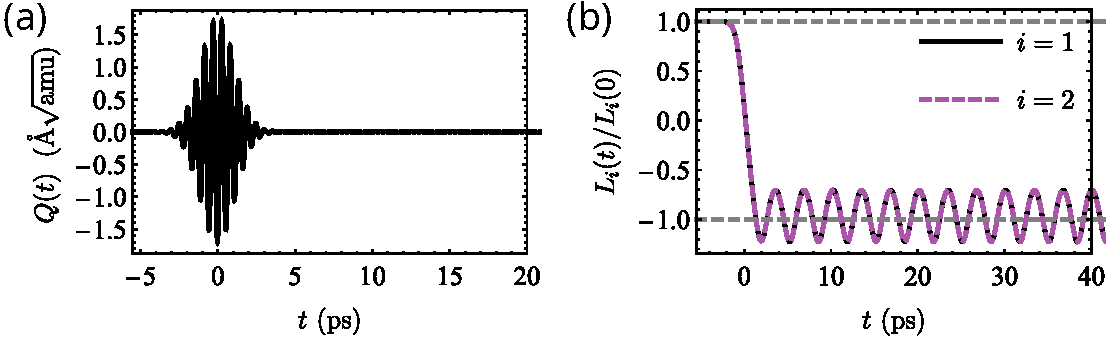
\includegraphics[width=\textwidth]{./gfx/ch6/nonequilibriumtheory1.pdf}
\captionsetup{singlelinecheck=off}
\caption[]{
\label{fig:nonequilibriumtheory1}
\begin{enumerate*}[label=\caplabel, ref=\capref]
\item Phonon mode and \item \gls{afm} \gls{op} following photo-excitation with coupling $(L_1^2 + L_2^2)(Q+Q^2)$.
\end{enumerate*}
}
\end{figure}

First, we assume that there is no strain in the sample.
The only term linking the \gls{afm} \gls{op} to the time-dependent phonon is $(L_1^2 + L_2^2)(Q+Q^2)$.
We find that this term can lead to flips of $L_1$ and $L_2$ by 180 degrees for long-enough laser pulses. \Cref{fig:nonequilibriumtheory1a} shows the phonon dynamics following photo-excitation with a $1$eV pulse and duration $\tau = 1.1$ \si{ps}.
The phonon frequency was assumed to be $\omega/(2\pi) = 3$ \si{THz}, and the initial temperature is $T=0$.     

\textit{Strain}

\begin{figure}
\centering{
\phantomsubfloat{\label{fig:nonequilibriumtheory2a}}
\phantomsubfloat{\label{fig:nonequilibriumtheory2b}}
}
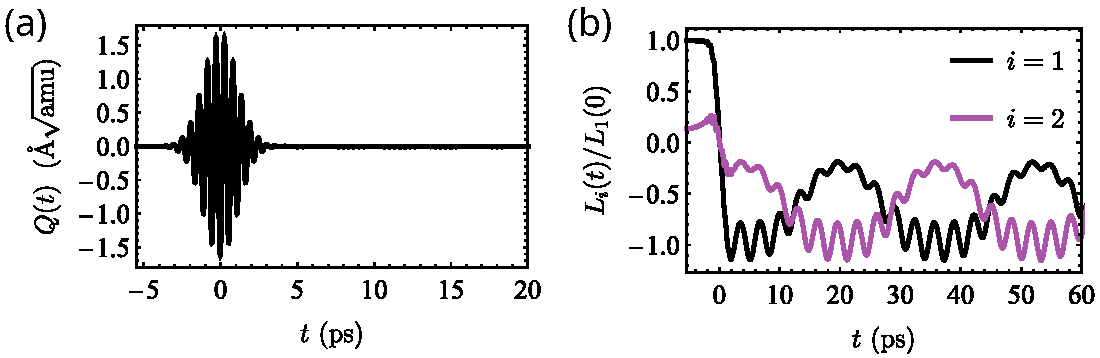
\includegraphics[width=\textwidth]{./gfx/ch6/nonequilibriumtheory2.pdf}
\captionsetup{singlelinecheck=off}
\caption[]{
\label{fig:nonequilibriumtheory2}
\begin{enumerate*}[label=\caplabel, ref=\capref]
\item Phonon mode and \item \gls{afm} \gls{op} following photo-excitation with coupling $L_1 L_2 e_2 Q$.
\end{enumerate*}
}
\end{figure}

The presence of strain mediates coupling terms between the phonon and the \gls{afm} \gls{op} that can lead to orientations absent in equilibrium.
In particular, the coupling term $L_1 L_2 e_2 Q$ induces a solution where the components $L_1, L_2$ oscillate around a position distinct to the initial configuration and to 180-degree flips.
We consider a pulse with duration $\tau = 1.2$ \si{ps}, phonon frequency $\omega/(2\pi) = 3$ \si{THz}, $T=0$, and strains $\epsilon_1 = 0.01$, $\epsilon_1 = 0.05$.
The long-time average of $L_2(t)$ acquires values comparable with $L_1(t)$, as seen in \cref{fig:nonequilibriumtheory2b}. 

\subsection{Nonviability of secondary order parameter in describing the \gls{rashg} data}\label{sec:alternativeinterpretation}

Using a combination of \gls{ptmb} and \gls{rashg}, we argue in the main text that, in equilibrium, the magnetism in \cmb that we observe is described by a spatial distribution of four domains $A$, $B$, $C$, and $D$, for which the order parameters satisfy the relations $l_A = -l_B$, $l_C = -l_D$, and $l_C = R(l_A)$, where $R$ is an element of the high-temperature point group \htpg.
In this scenario, the contrast in SHG between e.g. $l_A$ and $l_B$ comes from the fact that there can be two contributions to the \gls{rashg} signal which interfere with each other and transform differently as $l_A \rightarrow l_B$.
That is, we can write
\begin{equation}
I_\mathrm{SHG} \propto |e^\mathrm{out}_i \chi_{ijk} e^\mathrm{in}_j e^\mathrm{in}_k|^2,
\end{equation}
where
\begin{equation}
\begin{aligned}
\chi_{ijk} &\equiv &&\chione_{ijk} + \chitwo_{ijk}, \\
\end{aligned}
\end{equation}
\begin{equation}
\label{eq:trrelations}
\begin{aligned}
T (\chione_{ijk}) &= &-&\chione_{ijk}, \\
T (\chitwo_{ijk}) &= &&\chitwo_{ijk},
\end{aligned}
\end{equation}
$T$ is the time-reversal operator which takes $l_A \rightarrow -l_A = l_B$, and $e^\mathrm{in}$ and $e^\mathrm{out}$ are unit vectors in the direction of the polarization of the incoming and outgoing electric fields, respectively.

An important question thus arises: what is the origin of the two sources $\chione$ and $\chitwo$?
The simplest explanation is that both contributions are due to the \gls{afm} \gls{op}; the relations in \cref{eq:trrelations} are then permitted below $T_c$, where time-reversal symmetry is broken and so $\chi_{ijk}$ can, in general, have parts which transform as both even and odd under time-reversal.
However, an alternative interpretation is that there are in fact two \glspl{op} $l$ and $g$, with $g$ being e.g. some structural \gls{op}, so that, e.g.
\begin{equation}
\label{eq:proptolg}
\begin{aligned}
\chi^C &\propto l + g, \text{and} \\
\chi^D &\propto l + Rg,
\end{aligned}
\end{equation}
for some $R \in \htpgmathmode$.

In this interpretation, alternative descriptions of the time-resolved results, involving e.g. a melting of $g$ while the $l$ stays fixed, may explain \cref{fig2}, but not imply a reorientation of $l$ as we claim in the main text.
However, we argue that such an interpretation is not a viable description of our results, both in and out of equilibrium.
% The reasoning can be seen by considering the effect of \cref{eq:proptolg} on the \gls{rashg} patterns corresponding to domains $C$ and $D$ (see \cref{fig1} in the main text).
This can be understood by considering the fact that the \gls{rashg} pattern in \cref{fig1:f} has nodes at $\phi=0$ and $\phi=\pi$ for all temperatures below $T_c$ (see \supsupcref{ctempdep}).
In the case $Rg = -g$, this suggests that, if there are indeed two independent order parameters contributing to the \gls{rashg} pattern, their amplitudes must exactly cancel for all $T < T_c$.
This is unlikely as the two independent order parameters should in general depend differently on temperature.
Moreover, the case $Rg \neq -g$ is difficult to reconcile in light of the result that the \gls{ptmb} signal is invariant under thermal cycling.
In nonequilibrium, any scenario involving the melting of one \gls{op} while the other stays fixed must also be reconciled with the observation that the nodes in \cref{fig2:c} in the initial state (before $t=0$) become peaks in the final state.

Furthermore, the above interpretation must also explain how the final state of the transition seems to differ from sample to sample (as explained in the main text; see \supsupcref{CtoBshort,CtoBlong}), as well as how the \gls{rashg} is poled in equilibrium to only two of many different degenerate states.
Both of these facts fall out naturally from the assignment presented in the main text.

Together with the lack of a change in the \gls{xrd} across $T_c$ (see \supsupcref{xrd}), the above considerations suggest that the scenario presented in the main text, which neatly describes the data both in and out of equilibrium, is the most likely.
Future studies will be required to completely truly rule out all alternative scenarios.

\subsection{Fits to susceptibility tensors}\label{sec:fitting}

In the text, it was remarked that the \gls{op} assignment depicted in \crefrange{fig1}{fig2} was consistent with the \gls{shg} susceptibility tensors extracted by fitting the \gls{rashg} patterns.
In this section, we state how this fitting was performed.

Before that discussion, however, we must mention one important point about the predictive power of these fits.
Since the low-temperature point group of \cmb is $\bar{1}'$, the relevant susceptibility tensors are entirely unconstrained and the cost function to be minimized may involve upward of 36 free parameters.
Thus, in principle, many combinations of parameters may fit the data appropriately, thereby limiting the extent to which the \gls{shg} fits can be used to draw conclusions about the underlying state.
One must look to other arguments, e.g. involving \gls{ptmb}, to draw useful conclusions about the data, as was done in the text.
However, once a conclusion has been made, it can at least be checked that a set of fitting parameters \textit{does} exist that is consistent with the conclusion and with the data.
This is the goal of this section.

The \gls{op} assignment discussed in the text involves two parts.
In the first part, the equilibrium SHG in the four domains of \cref{fig1} is assigned to four different \gls{op} directions, in which the \gls{shg} on consecutive cooldowns on a single spot is due to $180^\circ$ \gls{afm} configurations, and adjacent spots have a relative angle between them.
As argued in the text, since the $180^\circ$ domains have different \gls{rashg} patterns, there are most likely two contributions to the \gls{shg} adding coherently to give an interference term, as observed in other magnetic systems\citep{fiebig_second_1994, fiebig_second_2001, fiebig_second-harmonic_2005}.
Designating the four configurations as $A$, $B$, $C$, and $D$ (for \cref{fig1:d}, \cref{fig1:e}, \cref{fig1:f}, and \cref{fig1:g}, respectively), we thus have
\begin{equation}
\begin{aligned}
\label{eq:equilibrium}
\chi^{A}_{ijk} &= &&&&\chione_{ijk}+\chitwo_{ijk}\\
\chi^{B}_{ijk} &= &&&-&\chione_{ijk}+\chitwo_{ijk}\\
\chi^{C}_{ijk} &= &&R(&&\chione_{ijk}+\chitwo_{ijk})\\
\chi^{D}_{ijk} &= &&R(&-&\chione_{ijk}+\chitwo_{ijk}),
\end{aligned}
\end{equation}
where $\chione$ is the susceptibility tensor related to the magnetic order\citep{fiebig_second-harmonic_2005}, $\chitwo$ is the susceptibility tensor corresponding to the secondary component discussed above, and $R(\cdot)$ refers to an operation by some element $R$ of the high-temperature point group ($\bar{3}m$), i.e.
\[
R(\chi_{ijk}) \equiv R_{il}R_{jm}R_{kn}\chi_{lmn}.
\]

In the time-resolved case, \ref{eq:equilibrium} should hold before zero delay, and a similar set of equations should hold after zero delay in the final state:

\begin{equation}
\begin{aligned}
\label{eq:nonequilibrium}
\chi^{A'}_{ijk} &= &&\alpha\chione_{ijk}+\chitwo_{ijk}\\
\chi^{B'}_{ijk} &= &-&\alpha\chione_{ijk}+\chitwo_{ijk}\\
\chi^{C'}_{ijk} &= &&\alpha\chione_{ijk}+\chitwo_{ijk}\\
\chi^{D'}_{ijk} &= &&\alpha\chione_{ijk}+\chitwo_{ijk}.
\end{aligned}
\end{equation}
Here, $\alpha$ is an overall factor to account for the fact that the magnitude of the \gls{op} may change due to heating following the transition.
We also allow a relative scale (close to unity) between $A$ / $B$ / $A'$ / $B'$ and $C$ / $D$ / $C'$ / $D'$ to account for the fact that these are taken on different spots on the sample.

\begin{figure}
\centering
\includegraphics[width=\textwidth]{./gfx/ch6/fitting.pdf}
\caption{
\label{fitting}
Fits to the \gls{rashg} pattern in the four domains of \cref{fig1} $2.0$ \si{ps} before ($A$, $B$, $C$, $D$) and $\apx 40$ \si{ps} after ($A'$, $B'$, $C'$, $D'$) zero delay.
Data is represented by black circles; solid lines are fits to \seqs{1}{2} with $\chitwo$ denoted in the legend.
}
\end{figure}

For $\chione_{ijk}$, we use the totally asymmetric complex electric dipole \gls{shg} tensor in the point group $\bar{1}'$, which has $36$ independent elements.
In the language of \citet{birss}, this would be referred to as a $c$-type tensor and should have purely imaginary components; however, in the presence of dispersion or dissipation, complex components are also allowed.
For $\chitwo_{ijk}$, many options are possible, including an $i$-type electric dipole component, electric quadrupole component, or magnetic dipole component, each of which may couple with the \gls{afm} \gls{op}.
With each of these options for $\chione$ and $\chitwo$, we fit the \gls{rashg} data at $\Delta t=-2$ \si{ps} and at long times ($\Delta t\approx 40$ \si{ps}).
It is found that all possibilities for $\chitwo$ produce an appropriate fit to the data (see \cref{fitting}).

\subsection{Error bar estimation for \cref{fluencedep}}

\begin{figure}
\centering
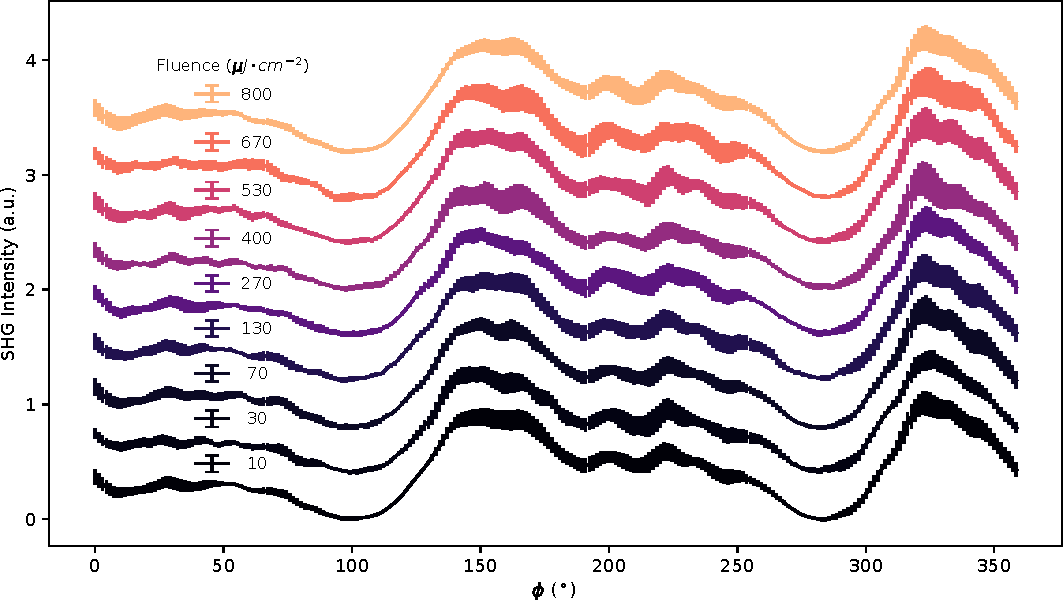
\includegraphics[width=\textwidth]{./gfx/ch6/errorbars.pdf}
\caption{\label{errorbars}\gls{rashg} results of \cref{fluencedep} depicted with estimated errorbars (see text).}
\end{figure}

The errorbars in \cref{errorbars} are ultimately due to uncertainty in the value of the \gls{shg} intensity at each angle $\phi$.
When these angles are integrated over, the associated uncertainties in the \gls{shg} intensity are summed in quadrature.
To extract the uncertainties in the \gls{shg} intensity as a function of angle is a somewhat difficult process, as these uncertainties are largely systematic rather than statistical.
Indeed, the \gls{rashg} pattern should in general be a smooth function of $\phi$; however, it is seen (e.g. \cref{fig2:d}) that the \gls{rashg} patterns are not necessarily smooth.
We therefore estimate the size of the errorbars using more heuristic methods, which, while imprecise, should at least give a rough approximation to the true uncertainty.

These heuristic errorbars in the \gls{shg} intensity are found by estimating the size of the variations in the \gls{rashg} pattern compared to a smoothed approximation (approximated with an $N=6$ FFT filter).
The errorbars computed this way are shown in \cref{errorbars}.

\begin{figure}
\centering
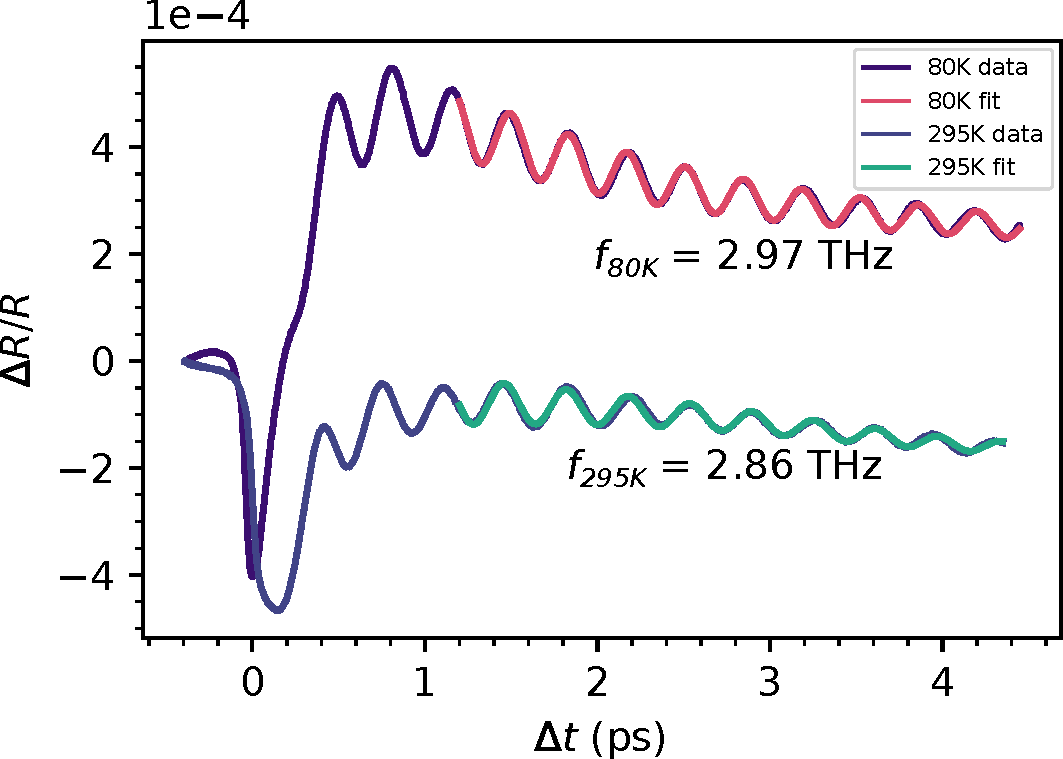
\includegraphics[width=\textwidth]{./gfx/ch6/pp.pdf}
\captionsetup{singlelinecheck=off}
\caption[]{
\label{pp}
Time-resolved reflectivity obtained from \cmb at $80$ \si{K} and $295$ \si{K}.
The pump and probe wavelengths were both $800$ \si{nm}, the pulse width was $28$ \si{fs}, and the pump and probe fluences were $10$ and $1$ \si{\mu J \cdot cm^{-2}}, respectively.
The data is windowed after the initial transients and then fit to a damped harmonic oscillator plus a polynomial background.
}
\end{figure}

\begin{figure}
\centering
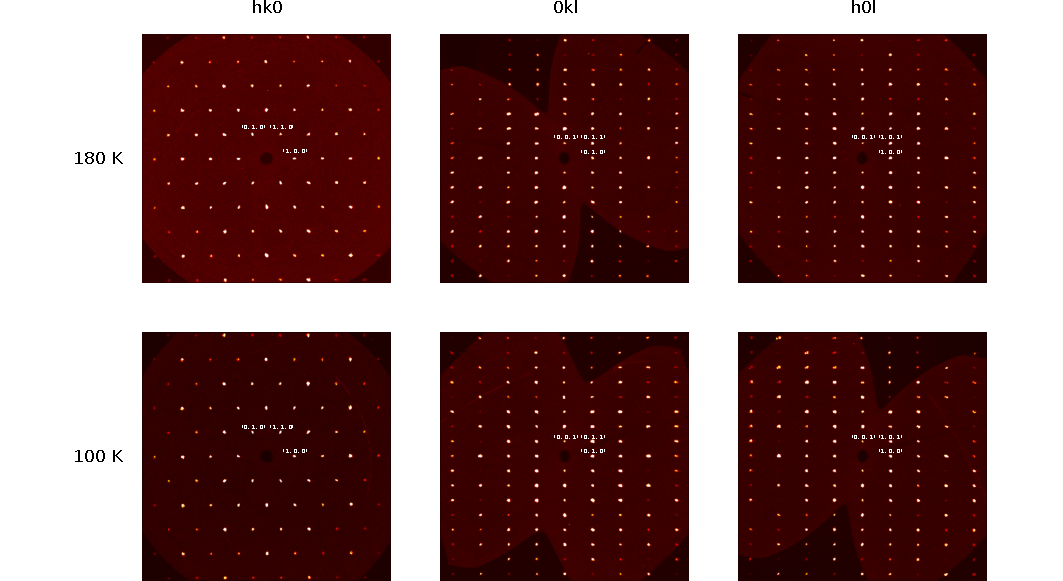
\includegraphics[width=\textwidth]{./gfx/ch6/xrd.pdf}
\captionsetup{singlelinecheck=off}
\caption[]{
\label{xrd}
Single-crystal \gls{xrd} precession images obtained from \cmb.
The high temperature refinement is in agreement with previous reports\citep{gibson_magnetic_2015}.
No change in the crystal structure is observed across $T_c=150$ \si{K}.
}
\end{figure}

\begin{figure}
\centering
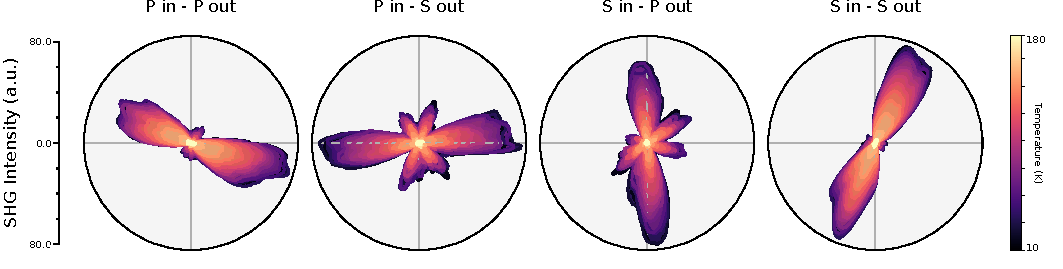
\includegraphics[width=\textwidth]{./gfx/ch6/full_fig0.pdf}
\caption{\label{fulltempdep}\gls{rashg} results of \cref{fig0} depicted in all four polarization channels (\PP, \PS, \SP, and \SS)}
\end{figure}

\begin{figure}
\centering{
\phantomsubfloat{\label{fullequilibrium:a}}
\phantomsubfloat{\label{fullequilibrium:b}}
\phantomsubfloat{\label{fullequilibrium:c}}
\phantomsubfloat{\label{fullequilibrium:d}}
\phantomsubfloat{\label{fullequilibrium:e}}
}
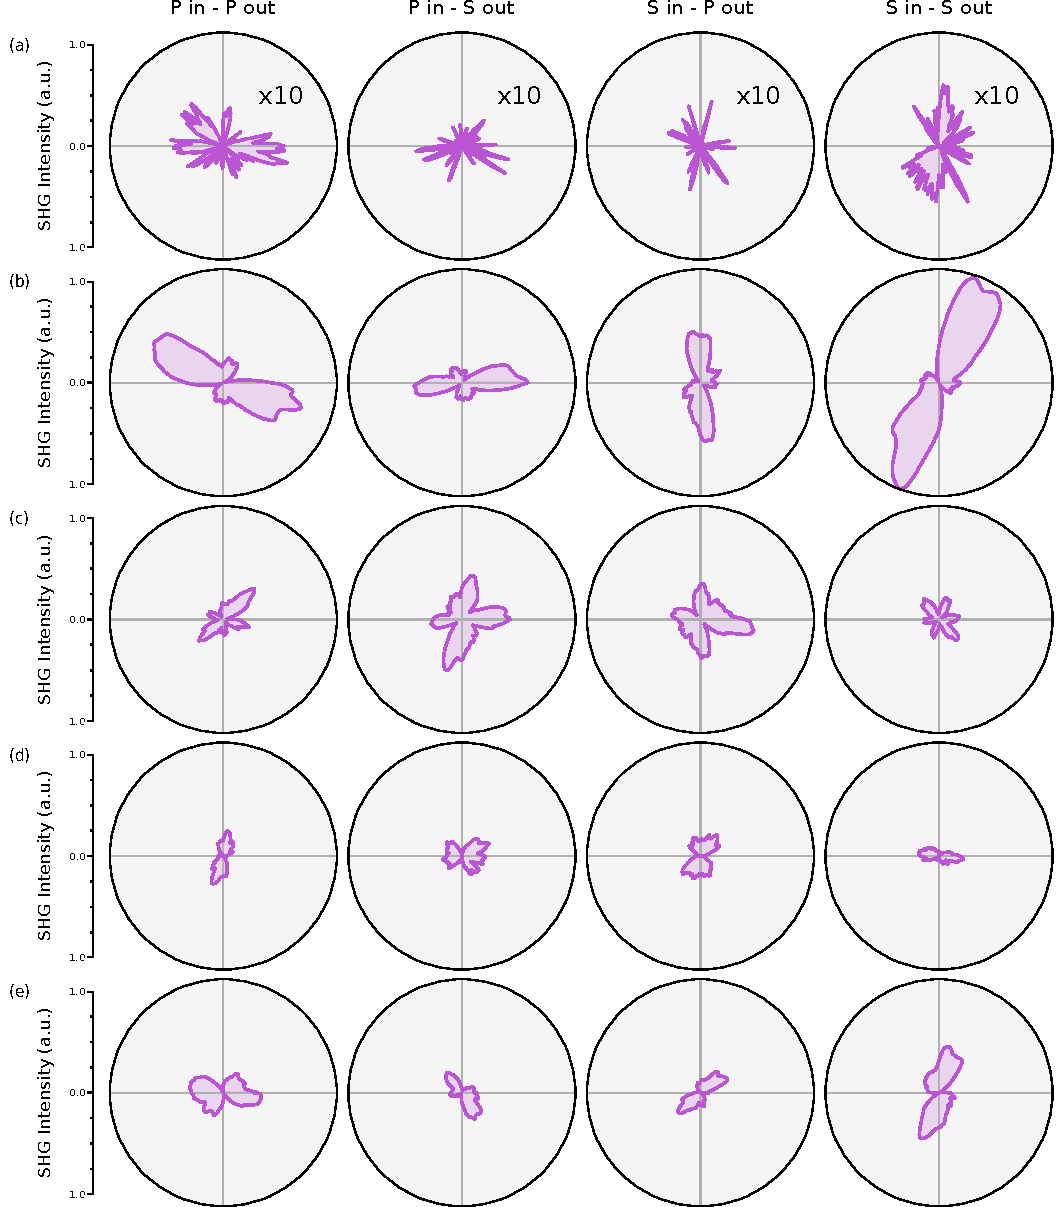
\includegraphics[width=\textwidth]{./gfx/ch6/full_fig1.pdf}
\captionsetup{singlelinecheck=off}
\caption[]{
\label{fullequilibrium}
\begin{enumerate*}[label=\caplabel, ref=\capref]
\item {} \item {} \item {} \item {} \item \gls{rashg} results of \cref{fig1:b,fig1:d,fig1:e,fig1:f,fig1:g} depicted in all four polarization channels (\PP, \PS, \SP, and \SS).
\end{enumerate*}
}
\end{figure}

\begin{figure}
\centering
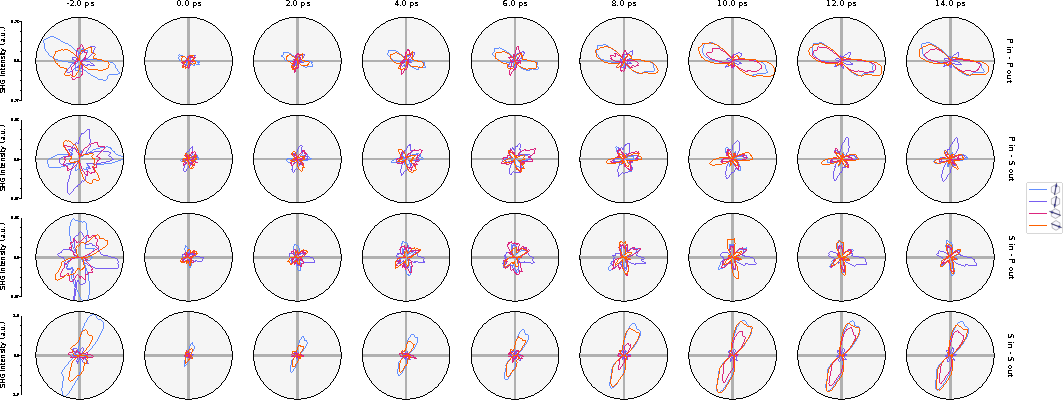
\includegraphics[width=\textwidth]{./gfx/ch6/full_fig2.pdf}
\caption{\label{fullnonequilibrium}\gls{rashg} results of \cref{fig2} depicted in all four polarization channels (\PP, \PS, \SP, and \SS).
The pump fluence is set to $\apx 600$ \si{\mu J \cdot cm^{-2}}.}
\end{figure}

\begin{figure}
\centering
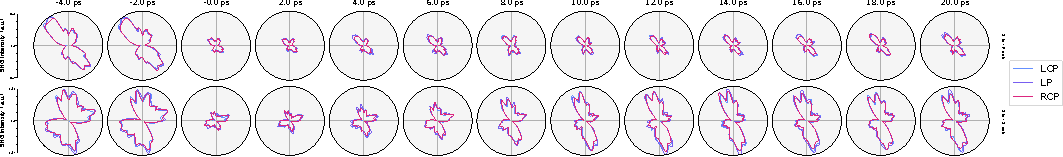
\includegraphics[width=\textwidth]{./gfx/ch6/polarization.pdf}
\caption{\label{polarization}\gls{rashg} results in a representative domain as a function of time for different pump polarization states (left circularly- (LCP), right circularly- (RCP), and linearly-polarized).
The pump fluence is set to $\apx 600$ \si{\mu J \cdot cm^{-2}}.
}
\end{figure}

\begin{figure}
\centering
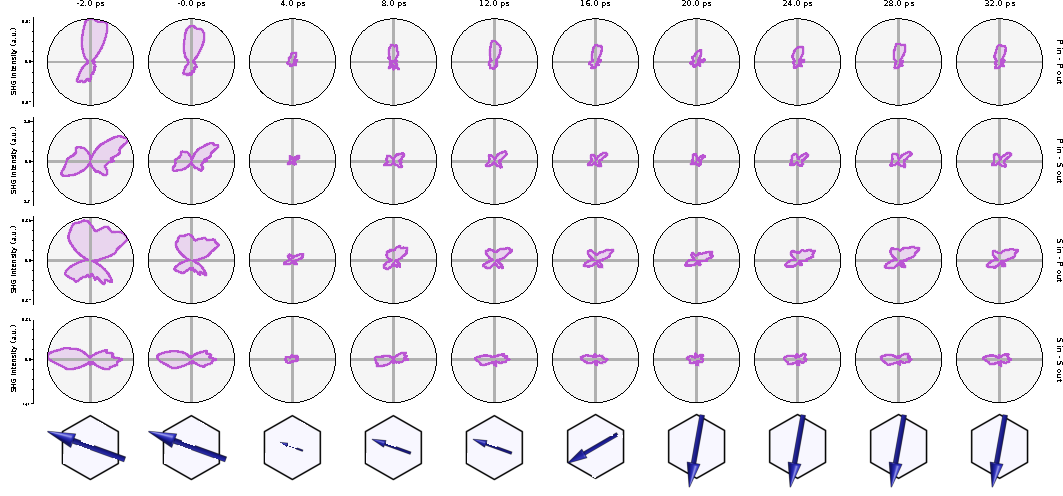
\includegraphics[width=\textwidth]{./gfx/ch6/C2B_short.pdf}
\caption{\label{CtoBshort}\gls{rashg} snapshots showing a transition to the state opposite to \figs{3}{c-d}.
The pump fluence is set to $\apx 600$ \si{\mu J \cdot cm^{-2}}.
\lastrow
The schematic representations beneath the \gls{rashg} plots are for illustration purposes only and the depicted angles are not quantitatively verified.
}
\end{figure}

\begin{figure}
\centering
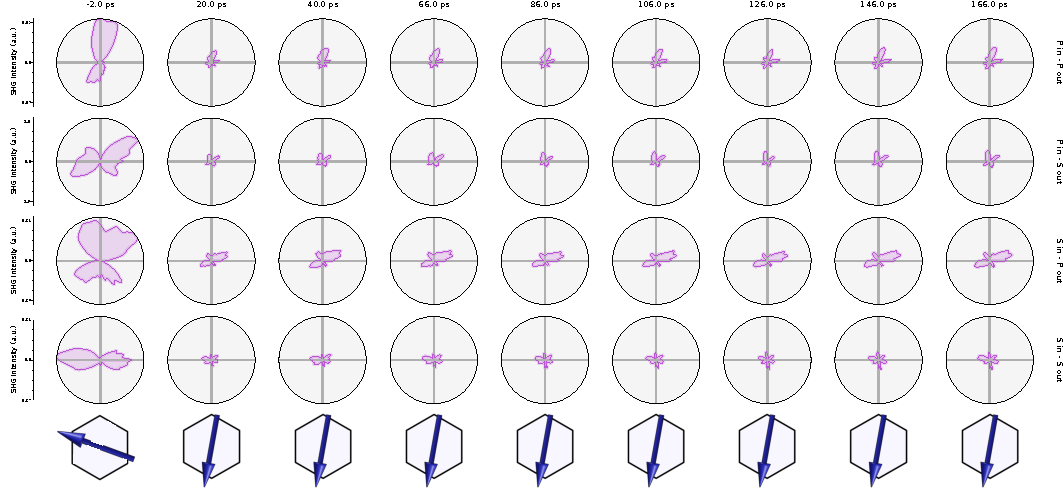
\includegraphics[width=\textwidth]{./gfx/ch6/C2B_long.pdf}
\caption{\label{CtoBlong}\gls{rashg} results in the same domain as \supsupcref{CtoBshort} plotted out to longer times.
The pump fluence is set to $\apx 600$ \si{\mu J \cdot cm^{-2}}.
\lastrow
The schematic representations beneath the \gls{rashg} plots are for illustration purposes only and the depicted angles are not quantitatively verified.
}
\end{figure}

\begin{figure}
\centering
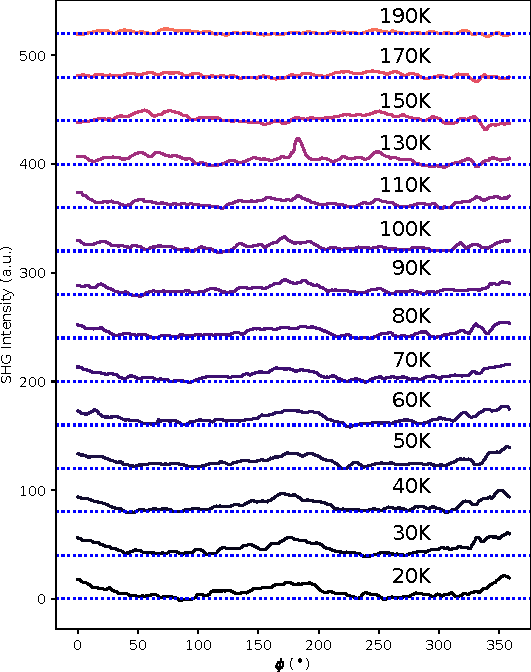
\includegraphics[width=\textwidth]{./gfx/ch6/ctempdep.pdf}
\caption{\label{ctempdep}
SHG intensity in the same domain as \cref{fig1:f} as a function of temperature.
}
\end{figure}
